\chapter{Arquitetura e implementação}
\label{cap:implementacao}

Numa primeira etapa, o desenvolvimento do trabalho teve como foco o Drools,
por permitir trabalhar diretamente com as regras de produção, memória de
trabalho, processamento temporal e atualização contínua do conhecimento ao
longo da simulação. Esta opção permitiu consolidar primeiro a arquitetura do
sistema, os factos, os eventos e as regras antes de avançar para a
representação equivalente em Prolog.

A componente em Prolog encontra-se ainda em desenvolvimento e deverá
reutilizar, tanto quanto possível, os mesmos conceitos e relações definidos
para a implementação com o Drools. O objetivo não é desenvolver duas soluções
completamente independentes, mas sim preservar a equivalência conceptual
entre os factos, regras e conclusões, tendo em conta as diferenças existentes
entre os dois paradigmas.

\section{Arquitetura e funcionamento}
\label{sec:arquitetura}

A arquitetura do sistema foi definida com o objetivo de separar o ambiente
onde decorre a simulação, a informação obtida através dos sensores e o
conhecimento utilizado pelo motor de inferência. Esta separação permite
distinguir aquilo que efetivamente existe no cenário daquilo que o sistema
conhece num determinado momento. Assim, um objeto pode estar presente no
ambiente sem que tenha ainda sido detetado e, como consequência, não deve
influenciar a tomada de decisão enquanto essa informação não for transmitida
através dos sensores. Neste sentido, o ambiente simulado representa o estado
do veículo e dos restantes elementos presentes no cenário, enquanto os
sensores são responsáveis por observar apenas a informação correspondente à
sua função e alcance. As observações obtidas são transformadas,
posteriormente, em factos que podem ser utilizados pelo motor de inferência.
Desta forma, evita-se que o sistema tenha acesso antecipado a toda a
informação existente no ambiente e mantém-se uma separação entre o estado
real da simulação, a perceção e o conhecimento utilizado na decisão.

Os factos considerados relevantes são mantidos na memória de trabalho, que
representa o conhecimento atual do sistema. Nesta memória podem existir
informações relacionadas, por exemplo, com a velocidade do veículo, o limite
de velocidade conhecido, a presença de um objeto, o estado de um semáforo ou
as condições meteorológicas. À medida que o cenário evolui e são recebidas
novas observações, os factos podem ser inseridos, atualizados ou removidos, o
que permite que a informação utilizada na inferência acompanhe a evolução da
situação. Neste sentido, os factos presentes na memória de trabalho não
correspondem a uma cópia completa do \texttt{WorldState}, ou seja,
representam apenas a informação que foi percecionada e considerada relevante
para o processo de inferência. Assim, mantém-se a distinção entre aquilo que
existe no ambiente simulado e aquilo que o motor de inferência conhece num
determinado momento. De uma forma simplificada, a \cref{tab:componentes}
apresenta os principais componentes presentes na arquitetura do sistema.

\begin{table}[H]
  \centering
  \caption{Principais componentes da arquitetura do sistema}
  \label{tab:componentes}
  \small
  \begin{tabularx}{\textwidth}{@{}L{5.4cm}VX@{}}
    \toprule
    \textbf{Componente} & \textbf{Função no sistema} \\
    \midrule
    Ambiente / \texttt{WorldState} & Representa o estado do veículo e dos
      restantes elementos presentes no cenário. \\ \linhasep
    \texttt{SimulationEngine} & Coordena os diferentes ciclos da simulação e a
      interação entre os principais componentes. \\ \linhasep
    \texttt{SensorManager} & Recolhe a leitura dos sensores. \\ \linhasep
    \texttt{EventRouter} & Encaminha os dados para o motor de inferência. \\ \linhasep
    Memória de trabalho / \texttt{KieSession} & Mantém os factos e eventos
      conhecidos pelo sistema e permite a avaliação das regras nos diferentes
      ciclos de inferência. \\ \linhasep
    Base de conhecimento & Contém as regras utilizadas para interpretar os
      factos e produzir propostas de decisão. \\ \linhasep
    \texttt{DecisionContext} & Recebe as diferentes propostas de decisão
      resultantes do processo de inferência. \\ \linhasep
    \texttt{DecisionActuator} & A decisão escolhida é atribuída à ação do
      veículo. \\ \linhasep
    Interface & Permite acompanhar a simulação, interagir com o sistema e
      visualizar a informação produzida. \\ \linhasep
    \texttt{WorldPhysicsEngine} & Atualiza a evolução física simplificada do
      veículo, nomeadamente, a respetiva posição e velocidade. \\ \linhasep
    \texttt{ExplanationTrace} / \texttt{WorkingMemoryInspector} & Permitem
      acompanhar a execução das regras, as alterações na memória de trabalho e
      a informação utilizada para reconstruir o processo de decisão. \\
    \bottomrule
  \end{tabularx}
\end{table}

O funcionamento do sistema é cíclico. Em cada ciclo, o estado do ambiente é
atualizado e os sensores recolhem nova informação de acordo com a situação
observada. Os eventos são encaminhados para o motor de inferência e utilizados
para atualizar o conhecimento presente na memória de trabalho. De seguida, as
regras cujas condições são satisfeitas são avaliadas e podem sugerir uma ou
mais propostas de ação. Contudo, quando existe mais do que uma proposta, estas
são posteriormente comparadas antes de ser selecionada a decisão final. A
ação escolhida é então aplicada ao comportamento do veículo e pode resultar em
alterações como a redução da velocidade, a paragem ou uma mudança de via. Uma
vez alterado o estado do veículo, os sensores passam a transmitir dados de uma
nova situação, e dá-se início a um novo ciclo de processamento. A relação
entre os componentes anteriores e o fluxo de informação no processo da tomada
de decisão pode ser representada através da \cref{fig:arquitetura}.

\begin{figure}[H]
  \centering
  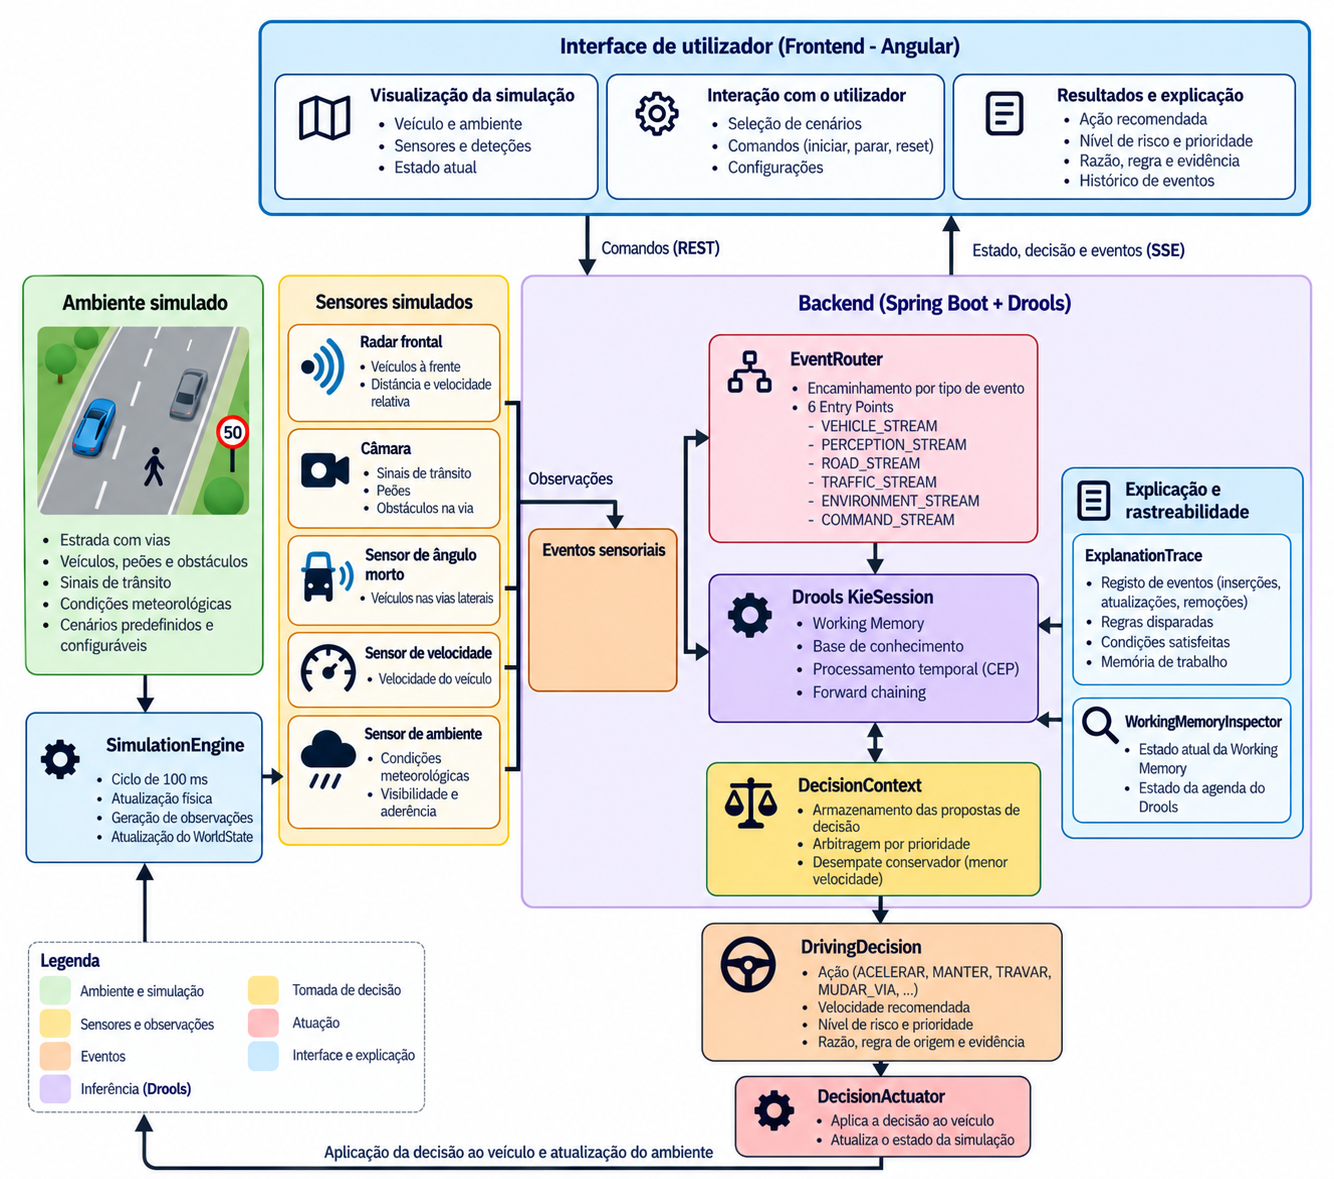
\includegraphics[width=\textwidth]{figuras/arquitetura-sistema.png}
  \caption{Arquitetura geral e fluxo de informação do sistema pericial}
  \label{fig:arquitetura}
\end{figure}

\FloatBarrier
\section{Tecnologias utilizadas}
\label{sec:tecnologias}

Até ao momento, o trabalho desenvolvido utiliza diferentes tecnologias de
acordo com a responsabilidade de cada componente do sistema. Neste sentido,
apresentam-se as principais tecnologias utilizadas na versão atual
(\cref{tab:tecnologias}).

\begin{table}[H]
  \centering
  \caption{Principais tecnologias utilizadas na implementação do sistema}
  \label{tab:tecnologias}
  \small
  \begin{tabularx}{\textwidth}{@{}L{3.3cm}VL{4.1cm}VX@{}}
    \toprule
    \textbf{Componente} & \textbf{Tecnologia} & \textbf{Utilização no projeto} \\
    \midrule
    \emph{Backend} & Java 17 e Spring Boot 3.3.4 & Simulação, sensores,
      integração com o motor de inferência e API \\ \linhasep
    Motor de inferência & Drools/KIE 8.44 & Memória de trabalho, regras DRL e
      \emph{forward chaining} \\ \linhasep
    \emph{Frontend} & Angular 18 e RxJS & Visualização e interação com o
      utilizador e apresentação do estado e das decisões \\ \linhasep
    Comunicação & REST e \emph{Server-Sent Events} (SSE) & Atualização
      contínua da interface e envio de comandos para o \emph{backend} \\ \linhasep
    Testes \emph{backend} & JUnit 5 & Testes para as regras e integração dos
      componentes utilizados \\ \linhasep
    Testes \emph{frontend} & Jasmine/Karma e Playwright & Testes unitários da
      interface e testes \emph{end-to-end} \\
    \bottomrule
  \end{tabularx}
\end{table}

\FloatBarrier
\section{Drools}
\label{sec:drools}

O Drools é, neste momento, o principal motor de inferência do sistema
desenvolvido. A respetiva utilização permite representar o conhecimento do
domínio através das regras declarativas e manter esta lógica separada dos
componentes responsáveis pela simulação, sensores e interface. A
implementação utiliza uma \texttt{KieSession} com estado, o que, por
consequência, permite manter factos na memória de trabalho nos diferentes
ciclos de inferência. Esta característica é necessária por se tratar de um
domínio dinâmico, uma vez que a informação não é fornecida toda de uma só
vez, ou seja, a informação que chega dos sensores pode alterar o conhecimento
disponível ao motor de inferência.

A criação e a gestão da sessão são asseguradas pela componente
\texttt{KnowledgeSession}. No início da simulação são introduzidos alguns
factos que representam o estado inicial conhecido pelo sistema como, por
exemplo, o limite de velocidade, as condições meteorológicas, a ocupação das
vias adjacentes e estados associados a diferentes elementos rodoviários. À
medida que a simulação evolui, estes factos podem ser atualizados ou
substituídos com base nas novas observações. Os eventos dados pelos sensores
são encaminhados para o Drools através do \texttt{EventRouter}, organizados em
diferentes \emph{entry points}, tendo em conta o tipo de informação
representada. Na implementação atual, encontram-se definidos seis fluxos
relacionados com o estado do veículo, perceção, elementos da estrada, controlo
de tráfego, ambiente e comandos. Esta organização permite separar
semanticamente os diferentes tipos de eventos e facilita a aplicação das
regras associadas a cada domínio de conhecimento. Por exemplo, medições
relativas à distância de um veículo da frente, à velocidade relativa e ao TTC
são encaminhadas para o fluxo de perceção, enquanto eventos relacionados com
sinais de trânsito ou obstáculos são encaminhados para o fluxo associado à
estrada.

O \texttt{EventRouter} organiza estes eventos, como referido, em seis
\emph{entry points} (\cref{tab:entry-points}), o que permite separar os
diferentes tipos de informação antes de ser utilizada pelas regras. Esta divisão facilita a identificação da
origem semântica dos eventos e permite que as regras utilizem apenas os
fluxos que são relevantes para cada situação.

\begin{table}[H]
  \centering
  \caption{\emph{Entry points} utilizados para encaminhar os eventos para o
    Drools}
  \label{tab:entry-points}
  \small
  \begin{tabularx}{\textwidth}{@{}L{4.6cm}VX@{}}
    \toprule
    \textbf{\emph{Entry point}} & \textbf{Exemplos de informação} \\
    \midrule
    \texttt{VEHICLE\_STREAM} & velocidade e estado do veículo \\ \linhasep
    \texttt{PERCEPTION\_STREAM} & distância frontal, velocidade relativa, TTC,
      ocupação de via e presença de peões \\ \linhasep
    \texttt{ROAD\_STREAM} & limites de velocidade, sinais STOP, obstáculos \\ \linhasep
    \texttt{TRAFFIC\_STREAM} & estado dos semáforos \\ \linhasep
    \texttt{ENVIRONMENT\_STREAM} & meteorologia, visibilidade e aderência \\ \linhasep
    \texttt{COMMAND\_STREAM} & pedidos de aceleração e mudança de via \\
    \bottomrule
  \end{tabularx}
\end{table}

Uma vez que a memória de trabalho deve acompanhar a evolução do ambiente,
parte da informação não pode manter-se válida indefinidamente. Na
implementação atual, vários factos associados às observações dos sensores
deixam de ser considerados quando não são atualizados durante aproximadamente
600~ms. Desta forma, evita-se que uma observação antiga continue a representar
uma situação que pode já não existir.

A base de conhecimento encontra-se em vários ficheiros DRL, organizados de
acordo com o tipo de situação a tratar. Na versão atual do projeto, existem
ficheiros direcionados, entre outros, à atualização dos estados, situações de
emergência, veículos à frente, peões, limites de velocidade, semáforos, sinais
de trânsito, mudança de via, perigos rodoviários, meteorologia e raciocínio
temporal. Esta separação foi uma decisão consciente para evitar a
concentração da lógica num único ficheiro e facilitar a localização e futura
alteração das regras associadas a cada situação.

Uma das opções definidas na implementação diz respeito a manter a lógica
associada à tomada de decisão nas regras do Drools, em vez de a distribuir por
estruturas condicionais no código Java ou na interface. Desta forma, os
componentes Java são responsáveis pela simulação, gestão do ambiente,
sensores, pelo encaminhamento dos eventos e pela aplicação das decisões,
enquanto o conhecimento utilizado para decidir é mantido, tanto quanto
possível, nos ficheiros de regras. A interface tem como função a interação e
visualização da simulação, mas não é responsável pela definição da política
de decisão. Esta separação permite distinguir a infraestrutura necessária ao
funcionamento do sistema do conhecimento do domínio e facilita a leitura,
alteração e validação das regras.

A versão atual tem cerca de 17 ficheiros DRL, com 77 regras, nomeadamente,
regras para a atualização do estado, validade da informação, decisão e
processamento temporal. Por outras palavras, uma regra em Drools verifica os
factos ou eventos disponíveis e, caso as respetivas condições sejam
satisfeitas, pode fazer uma nova proposta de decisão. Neste sentido, estamos
perante a lógica de \emph{forward chaining}: alterações nos factos disponíveis
podem influenciar que novas regras sejam aplicadas, tendo em conta os dados
recebidos durante a execução da simulação. O recurso a este tipo de lógica
adequa-se ao funcionamento do sistema, uma vez que a inferência é desencadeada
pela chegada e atualização contínua de informação. À medida que novos eventos
e factos são introduzidos ou alterados, podem ser aplicadas novas regras que,
como consequência, poderão dar origem a novas conclusões ou propostas de
decisão. Esta abordagem distingue-se de um processo orientado por uma única
consulta, uma vez que o contexto de decisão evolui continuamente durante a
simulação.

Para além da aplicação das regras, o sistema necessita de selecionar uma
decisão quando existem várias propostas no mesmo ciclo de inferência. Esta
função é feita através do \texttt{DecisionContext}. No início de cada ciclo é
definida uma decisão base e, à medida que as regras levam a novas propostas,
estas são comparadas através da respetiva prioridade. Uma proposta substitui a
anteriormente considerada quando apresenta uma prioridade superior. Em
situações de igualdade de prioridade, aplica-se o critério de desempate
descrito na \cref{sec:prioridades}. Depois de concluída esta comparação, a proposta selecionada é aplicada a um
objeto \texttt{DrivingDecision}, que guarda a informação associada à decisão
final, nomeadamente a ação, a velocidade recomendada, o nível de risco, a
prioridade, a razão apresentada, a regra que lhe deu origem, o instante da
decisão e a evidência utilizada. Posteriormente, a decisão é executada pelo
\texttt{DecisionActuator}, responsável por traduzir a decisão selecionada numa
alteração no comportamento do veículo. Esta alteração modifica o estado da
simulação e influencia as leituras dos sensores nos ciclos seguintes.

O ciclo base da simulação utiliza um passo de 100~ms. Assim, associado à
\texttt{KieSession} existe um relógio que acompanha estes ciclos, de forma
coordenada. Desta forma, o tempo considerado pelo motor de inferência evolui
em conjunto com os diferentes ciclos, o que possibilita não só avaliar, como
também reproduzir as janelas utilizadas pelas regras, independentemente do
tempo real da execução da aplicação.

Por último, para a implementação foi utilizado o \emph{Complex Event
Processing} (CEP), que permite tratar determinados dados como eventos e ter em
conta a respetiva dimensão temporal. Em vez de avaliar apenas uma observação
isolada, podem ser utilizadas janelas que mantêm um conjunto de
acontecimentos recentes para análise. No presente trabalho, este mecanismo é
utilizado, por exemplo, através de uma janela temporal de dois segundos para
observações relacionadas com o TTC e de uma janela com base nas cinco
observações mais recentes para analisar a informação associada à distância
frontal. Desta forma, as regras podem considerar não apenas o valor atual, mas
também a persistência ou evolução recente de uma determinada condição. A
título de exemplo, relativamente ao TTC, considera-se que uma das regras
procura pelo menos duas observações com um valor inferior a 2,5 segundos numa
janela temporal de dois segundos (\cref{sec:raciocinio-temporal}). Assim, ter apenas uma observação reduzida
não é o suficiente para caracterizar, por si só, uma situação como
persistente. Por outro lado, quando o TTC apresenta um valor inferior a 1,3
segundos, existe uma condição de reação imediata, uma vez que aguardar por
novas observações pode ser prejudicial para a tomada de decisão imediata.
Assim, o sistema distingue entre a repetição de uma situação de risco ao longo
das observações recentes e uma situação de maior urgência que pode justificar
uma resposta imediata.

Neste sentido, a implementação em Drools não corresponde só a um conjunto
isolado de regras. O motor de inferência encontra-se integrado num ciclo
contínuo, em que os eventos atualizam o conhecimento disponível e as regras
resultam em propostas que, após serem comparadas, levam à proposta da tomada
de decisão e, consequentemente, provocam efeitos no estado do veículo.

\section{Prolog}
\label{sec:prolog}

A implementação em Prolog corresponde à segunda fase do desenvolvimento do
sistema e encontra-se, atualmente, em desenvolvimento inicial. Ao ser
implementado, irá permitir a representação do mesmo conhecimento através de
um paradigma lógico. Neste sentido, pretende-se reutilizar conceitos como os
estados do veículo e do ambiente, os diferentes elementos rodoviários, as
condições necessárias para determinada decisão e as conclusões inferidas pelo
sistema. Os factos representados em Prolog deverão, sempre que possível,
corresponder aos mesmos conceitos utilizados na memória de trabalho do
Drools, enquanto as regras deverão preservar o significado das condições e
conclusões definidas na base de conhecimento. No entanto, a implementação em
Prolog não é uma simples tradução sintática dos ficheiros DRL. Será
necessário analisar de que forma conceitos como estado mutável, informação
temporal, prioridades e explicação podem ser representados de forma
equivalente dentro do paradigma lógico.

Nesta fase, o objetivo principal consiste em assegurar que os dois sistemas
partilhem a mesma interpretação do domínio. Para os mesmos factos relevantes,
deverá ser possível obter conclusões conceptualmente equivalentes, ainda que o
processo interno utilizado para chegar a essas conclusões seja diferente. A
comparação entre as duas implementações será aprofundada à medida que a
componente em Prolog for concluída, com o objetivo de analisar as diferenças
entre uma abordagem baseada em regras de produção e uma abordagem baseada em
inferência lógica.

\section{Estado atual do protótipo}
\label{sec:estado-prototipo}

A \cref{tab:estado-prototipo} resume o estado atual do protótipo face ao
modelo descrito nos capítulos anteriores, distinguindo os mecanismos já
implementados dos que estão apenas previstos.

\begin{table}[H]
  \centering
  \caption{Estado atual do protótipo}
  \label{tab:estado-prototipo}
  \small
  \begin{tabularx}{\textwidth}{@{}>{\raggedright\arraybackslash}XV
      L{2.3cm}VL{6.2cm}@{}}
    \toprule
    \textbf{Mecanismo} & \textbf{Estado} & \textbf{Observação} \\
    \midrule
    Radar frontal, câmara, radares de canto, velocidade e sensor de ambiente
      & Implementado & Sensores simulados \\ \linhasep
    LiDAR, sensor de ângulo da direção e sensor de luminosidade
      & Previsto & -- \\ \linhasep
    Raciocínio temporal (janelas CEP)
      & Implementado & TTC e distância ao veículo da frente \\ \linhasep
    Validade das perceções
      & Implementado & Expiram ao fim de cerca de 600~ms sem atualização \\ \linhasep
    Níveis de risco e categorias de prioridade
      & Implementado & Quatro níveis de risco e sete categorias \\ \linhasep
    Resolução de conflitos e desempate
      & Implementado & Desempate pela menor velocidade recomendada \\ \linhasep
    Criticidade pela distância de travagem (\cref{eq:dtrav})
      & Previsto & O protótipo usa limiares fixos de TTC e de distância \\ \linhasep
    Intervalo temporal (THW) e tempo até transpor a marca rodoviária (TLC)
      & Previsto & -- \\ \linhasep
    Nível de confiança das deteções
      & Previsto & -- \\ \linhasep
    Confirmação entre sensores e LiDAR como terceira fonte
      & Previsto & -- \\ \linhasep
    Paragem perante a falha de um sensor
      & Previsto & -- \\ \linhasep
    Explicações \emph{Why} e \emph{How}
      & Implementado & Regra de origem, razão, evidência e registo da
        execução \\ \linhasep
    Explicação \emph{Why Not}
      & Parcial & As propostas não selecionadas ainda não são guardadas \\ \linhasep
    Implementação em Prolog
      & Previsto & Em fase inicial \\
    \bottomrule
  \end{tabularx}
\end{table}
